% !TeX root = ../main.tex

\chapter{研究方法}

本章詳述本研究所採用的模型架構與評估方法，包含系統整體架構、食譜知識圖譜的建構流程、KGAT 模型的數學形式化、訓練策略，以及基於忠實度指標的可解釋性評估框架。

\section{系統架構}

本研究之系統架構可分為四個階段：(1) 資料預處理與知識圖譜建構：將 Food.com 原始資料轉化為結構化的協同知識圖譜；(2) 模型訓練：在協同知識圖譜上訓練 KGAT 模型，學習使用者與食譜的高品質嵌入表示；(3) 推薦生成：基於學習到的嵌入，為每位使用者生成 Top-$K$ 推薦清單；(4) 可解釋性評估：透過注意力路徑萃取與忠實度指標量化，驗證推薦結果的可解釋性。

\begin{figure}[htbp]
  \centering
  \includestandalone{figures/system_architecture}
  \caption{系統架構示意圖}
  \label{fig:system_architecture}
\end{figure}

\section{資料預處理與知識圖譜建構}

\subsection*{Food.com 資料集}

本研究採用 Food.com 食譜推薦資料集~\cite{majumder2019foodcom}，該資料集包含使用者對食譜的評分紀錄、食譜的詳細屬性（包含食材、標籤、營養成分等）。經過預處理後，我們將其轉化為隱式回饋形式——即僅保留使用者是否與食譜互動過的二元訊號，不區分評分高低。

\subsection*{協同知識圖譜 (CKG) 建構}

遵循 KGAT~\cite{wang2019kgat} 的設計理念，我們將使用者-食譜互動圖與食譜知識圖譜統一為一個協同知識圖譜 $\mathcal{G}$。具體而言：

\begin{figure}[htbp]
  \centering
  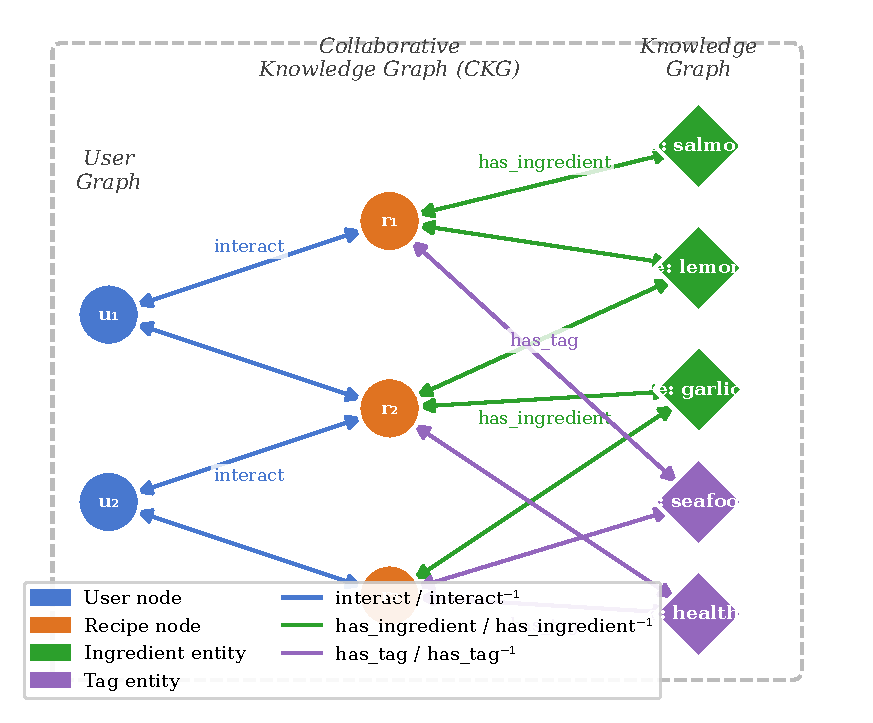
\includegraphics[width=0.82\linewidth]{figures/fig_ckg_schema.pdf}
  \caption{協同知識圖譜 (CKG) 架構示意：整合使用者-食譜互動圖與食譜知識圖譜，包含互動、食材與標籤三類關係邊。}
  \label{fig:ckg_schema}
\end{figure}

\begin{enumerate}[leftmargin=2em]
  \item \textbf{互動圖：}若使用者 $u$ 在訓練集中曾與食譜 $v$ 互動（例如收藏或評分），則建立邊 $(u, \text{interact}, v)$。測試集中的互動不納入 CKG，以避免資訊洩漏。
  \item \textbf{食譜屬性圖：}將食譜的標籤（如 \texttt{breakfast}、\texttt{chicken}、\texttt{weeknight}）與食材等屬性作為知識圖譜中的實體節點，並建立對應的關係邊，共形成食材（\texttt{has\_ingredient}）與標籤（\texttt{has\_tag}）兩類知識關係。例如，「食譜 A 包含食材 chicken」表示為三元組 $(v_A, \text{has\_ingredient}, e_\text{chicken})$。
  \item \textbf{反向邊擴充：}為確保訊息的雙向傳播，對每條邊 $(h, r, t)$ 均建立其反向邊 $(t, r^{-1}, h)$。
\end{enumerate}

最終建構的 CKG 包含使用者節點、食譜節點與屬性實體節點三類節點，以及互動關係與知識關係兩類邊。

\subsection*{超級節點修剪 (Super-node Pruning)}
  \label{sec:supernode_pruning}

在建構知識圖譜三元組之前，本研究先對高頻屬性實體進行超級節點修剪，以避免過度通用的節點在訊息傳播過程中引入大量雜訊路徑。

\begin{itemize}[leftmargin=2em]
  \item \textbf{食材超級節點：}統計所有食材的出現頻率後，移除出現頻率排名前 0.5\% 的高頻食材，以及根據先驗常識加入的基礎調味料（如 \texttt{salt}、\texttt{water}、\texttt{butter}、\texttt{sugar}、\texttt{eggs} 等）。兩部分取聯集後，共排除 74 個食材實體（詳細清單見附錄~\ref{app:preprocessing}）。這些食材出現在絕大多數食譜中，若納入 KG 將成為連結數萬節點的超級節點，其嵌入幾乎無法攜帶具有區辨力的語義資訊。
  \item \textbf{標籤超級節點：}統計所有標籤的出現頻率後，移除出現頻率排名前 50 的高頻標籤（如 \texttt{easy}、\texttt{healthy}、\texttt{main-dish} 等），這些標籤涵蓋面過廣，無法有效區分食譜的特色屬性。
\end{itemize}

此設計決策的理論依據在於：超級節點因與大量節點相連，其在 GNN 訊息傳播中相當於一個「資訊匯流點」，會造成鄰近節點的嵌入趨於相似（過度平滑）~\cite{li2018deeper}，並嚴重放大 §\ref{sec:kg_ablation} 所述的「淺層知識圖譜資訊汙染」效應。修剪後的知識圖譜保留語義區辨力強的屬性實體，使得實體間的關聯更能反映食譜的獨特風味特色。

\section{知識圖譜注意力網路 (KGAT)}

KGAT 模型由三個核心元件構成：嵌入層 (Embedding Layer)、注意力傳播層 (Attentive Propagation Layer) 與預測層 (Prediction Layer)。

\subsection*{嵌入層}

嵌入層將 CKG 中的每個節點與每條關係映射至 $d$ 維的稠密向量空間。對於節點 $i \in \mathcal{U} \cup \mathcal{V} \cup \mathcal{E}$，其初始嵌入為 $\bm{e}_i^{(0)} \in \mathbb{R}^d$；對於關係 $r \in \mathcal{R}$，其嵌入為 $\bm{e}_r \in \mathbb{R}^d$。

\subsection{Relation-Aware Attention 機制}

KGAT 的核心創新在於其關係感知的注意力機制。對於 CKG 中的一條邊 $(h, r, t)$，注意力分數的計算過程如下：

首先，計算三元組的原始注意力分數：
\begin{equation}
  \pi(h, r, t) = (\bm{W}_r \bm{e}_t)^\top \tanh \left( \bm{W}_r \bm{e}_h + \bm{e}_r \right)
  \label{eq:attention_raw}
\end{equation}
其中 $\bm{W}_r \in \mathbb{R}^{d' \times d}$ 為關係 $r$ 的轉換矩陣。此公式考慮了頭實體 $h$、關係 $r$ 與尾實體 $t$ 之間的語義相容性。

接著，透過 Softmax 歸一化得到最終的注意力權重：
\begin{equation}
  \alpha_{(h,r,t)} = \frac{\exp\left(\pi(h,r,t)\right)}{\sum_{(h,r',t') \in \mathcal{N}_h} \exp\left(\pi(h,r',t')\right)}
  \label{eq:attention_softmax}
\end{equation}
其中 $\mathcal{N}_h$ 表示節點 $h$ 在 CKG 中的所有鄰居三元組集合。

\subsection{Bi-Interaction 聚合機制}

在計算注意力權重後，KGAT 採用雙向互動 (Bi-Interaction) 聚合機制來更新節點表示。對於目標節點 $h$ 的第 $l$ 層嵌入更新：

首先計算注意力加權的鄰居聚合向量：
\begin{equation}
  \bm{e}_{\mathcal{N}_h}^{(l)} = \sum_{(h,r,t) \in \mathcal{N}_h} \alpha_{(h,r,t)} \cdot \bm{e}_t^{(l-1)}
  \label{eq:neighbor_agg}
\end{equation}

接著，透過加和（加性）與逐元素相乘（乘性）兩種互動方式組合：
\begin{equation}
  \bm{e}_h^{(l)} = \text{LeakyReLU}\left(\bm{W}_1^{(l)} \left(\bm{e}_h^{(l-1)} + \bm{e}_{\mathcal{N}_h}^{(l)}\right) + \bm{W}_2^{(l)} \left(\bm{e}_h^{(l-1)} \odot \bm{e}_{\mathcal{N}_h}^{(l)}\right)\right)
  \label{eq:bi_interaction}
\end{equation}
其中 $\bm{W}_1^{(l)}, \bm{W}_2^{(l)} \in \mathbb{R}^{d_l \times d_{l-1}}$ 為可學習的權重矩陣，$\odot$ 表示逐元素相乘 (Hadamard Product)。加性部分捕捉節點自身特徵與鄰居特徵的累積效果；乘性部分則能放大強烈相關的特徵維度、抑制不相關的雜訊。

經過 $L$ 層傳播後，將各層的嵌入進行拼接 (Concatenation) 以保留多尺度特徵：
\begin{equation}
  \bm{e}_h^* = \bm{e}_h^{(0)} \| \bm{e}_h^{(1)} \| \cdots \| \bm{e}_h^{(L)}
  \label{eq:concat}
\end{equation}

此設計等同於跳躍連接 (Skip Connection)，能有效緩解深層圖神經網路的過度平滑 (Over-smoothing) 問題~\cite{li2018deeper}。

\subsection*{預測層}

最終的使用者-物品偏好分數透過內積運算得出：
\begin{equation}
  \hat{y}_{uv} = {\bm{e}_u^*}^\top \bm{e}_v^*
  \label{eq:prediction}
\end{equation}

\begin{figure}[htbp]
  \centering
  \includestandalone{figures/kgat_architecture}
  \caption{KGAT 模型架構示意圖}
  \label{fig:kgat_architecture}
\end{figure}

\section{損失函數與模型訓練}

\subsection*{BPR 損失函數}

本研究採用貝葉斯個人化排序 (BPR)~\cite{rendle2009bpr} 作為訓練損失函數。BPR 假設使用者對已互動物品（正樣本 $v^+$）的偏好應高於隨機抽樣的未互動物品（負樣本 $v^-$）：
\begin{equation}
  \mathcal{L}_\text{BPR} = - \sum_{(u, v^+, v^-)} \ln \sigma\left(\hat{y}_{uv^+} - \hat{y}_{uv^-}\right) + \lambda \|\Theta\|_2^2
  \label{eq:bpr_loss}
\end{equation}
其中 $\sigma(\cdot)$ 為 Sigmoid 函數，$\lambda \|\Theta\|_2^2$ 為 L2 正則化項，$\Theta$ 為模型的所有可學習參數。

\subsection*{訓練策略}

模型使用 Adam 優化器進行訓練，並搭配 StepLR 學習率排程器進行學習率衰減。為支援在 Intel Arc GPU (XPU) 上高效訓練，本研究採用 BFloat16 混合精度訓練，並使用梯度檢查點 (Gradient Checkpointing) 技術緩解深層模型的記憶體壓力。

\section{可解釋性評估框架 (Fidelity)}

本研究建構了一套基於忠實度 (Fidelity) 指標的可解釋性評估框架，用於量化注意力路徑對模型預測的實際影響力。

\subsection*{注意力路徑萃取}

解釋路徑的萃取基於 KGATAttentionExplainer 模組，其運作流程如下：

\begin{enumerate}[leftmargin=2em]
  \item \textbf{全局注意力提取：}對訓練好的模型進行一次正向傳播，擷取每層 GNN 的注意力權重矩陣，並計算跨層平均值作為全局邊重要性指標。
  \item \textbf{路徑搜尋：}從使用者節點出發，沿 CKG 的拓撲結構搜尋所有連接至目標推薦物品的路徑（限制最大跳數為 $L$）。
  \item \textbf{路徑評分：}對每條路徑上所有邊的注意力權重進行連乘（聯合機率），得到該路徑的整體重要性分數：
    \begin{equation}
      \text{Score}(\text{path}) = \prod_{(h,r,t) \in \text{path}} \alpha_{(h,r,t)}
      \label{eq:path_score}
    \end{equation}
  \item \textbf{Top-$K$ 篩選：}依路徑分數排序，保留前 $K$ 條路徑作為最終解釋。
\end{enumerate}

\subsection*{Fidelity 量化指標}

給定使用者 $u$ 與推薦物品 $v$，令 $S$ 為所萃取的解釋路徑邊集合，$p_{uv}$ 為原始預測機率：

\begin{itemize}[leftmargin=2em]
  \item \textbf{Fidelity$^+$（必要性忠實度）：}移除 $S$ 中的邊後重新預測，計算機率降幅：
    \begin{equation}
      F^+ = p_{uv} - p_{uv \setminus S}
      \label{eq:fidelity_plus}
    \end{equation}
    $F^+ > 0$ 表示移除這些邊後模型信心下降，證明它們對預測有正向貢獻。

  \item \textbf{Fidelity$^-$（充分性忠實度）：}僅保留 $S$ 中的邊後重新預測，計算機率降幅：
    \begin{equation}
      F^- = p_{uv} - p_{uv|S}
      \label{eq:fidelity_minus}
    \end{equation}
    $F^- \approx 0$ 表示僅靠這些邊即可維持原預測，證明它們涵蓋了決策所需的充分資訊。
\end{itemize}

理想的解釋路徑應滿足 $F^+ \gg 0$（高必要性）且 $F^- \approx 0$（高充分性）。
